\section{\rqthree}

Here we investigate the impact of the composition of program variants into multivariant binaries.
To answer this research question, we create multivariant binaries from the program variants generated for the \corpussodium and the \corpusqrcode corpora. Then, we deploy the multivariant binaries into the Edge and collect their function call traces and execution times. 

\subsection*{Timing side-channels at program level.}

We compare the execution time distributions for each program for the original and the multivariant binary. All distributions are measured on 100k executions.
% statistics
We have observed that the distributions for multivariant binaries have a higher standard deviation of execution time.
A statistical comparison between the execution time distributions confirms the significance of this difference (P-value = 0.05 with a  Mann-Withney U test). This hints at the fact that the execution time for multivariant binaries is more unpredictable than the time to execute the original binary. 


% Curve flatenning
In \autoref{rq3:diversity:times}, each subplot represents the distribution for a single program, with the colors blue and green representing the original and multivariant binary, respectively. These plots reveal that the execution times are spread over a more extensive range of values than the original binary. 
This is evidence that execution time is less predictable for multivariant binaries than original ones.

\begin{figure*}[h]
    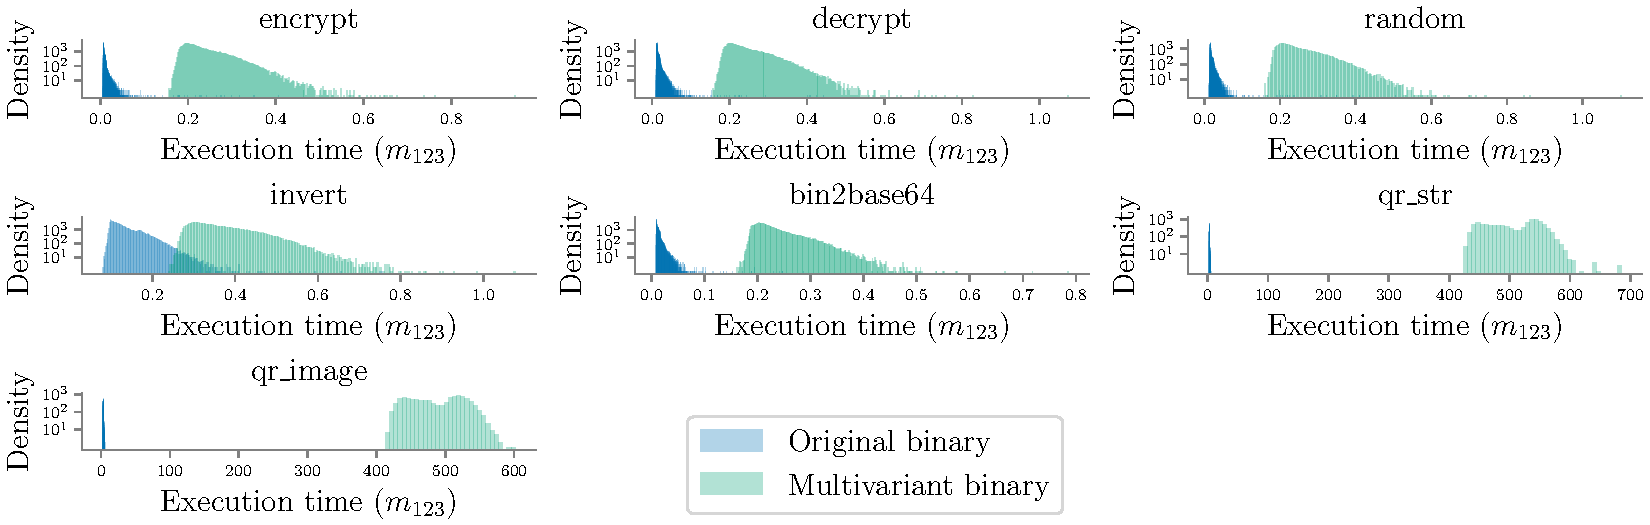
\includegraphics[width=\linewidth]{plots/times.pdf}
    \caption{Execution time distributions. Each subplot represents the distribution for a single program, blue for the original program and green for the multivariant binary. The X axis shows the execution time in milliseconds and the Y axis shows the density distribution in logarithmic scale.}
    \label{rq3:diversity:times}
\end{figure*}

Recall that the choice of function variant is randomized at each function invocation, and the variants have different execution times due to the code transformations, i.e., some variants execute more instructions than others. 
Consequently, attacks relying on measuring precise execution times \cite{blackhatpaper} of a function are made a lot harder to conduct as the distribution for the multivariant binary is different and even more spread than the original one.

\section{Answer to RQ3.}


The execution time distributions are significantly different between the original and the multivariant binary. Furthermore, no specific variant can be inferred from execution times gathered from the multivariant binary. Therefore, we contribute to mitigate potential attacks based on predictable execution times.